\documentclass{jarticle}
\usepackage{amsmath, amssymb}
\usepackage[dvipdfmx]{graphicx}

\title{組合せ論(ヴァン・リント&ウィルソン) 問題}

\newcommand{\N}{\mathbb{N}}
\newcommand{\Z}{\mathbb{Z}}
\newcommand{\Q}{\mathbb{Q}}
\newcommand{\R}{\mathbb{R}}
\newcommand{\C}{\mathbb{C}}
\newcommand{\F}{\mathbb{F}}

\newcommand{\comb}[2]{{}_{#1}\mathrm{C}_{#2}}

\renewcommand{\labelenumi}{(\roman{enumi})}
\renewcommand\thesubsection{\Alph{subsection}}

\begin{document}

\maketitle

\section{グラフ}
\subsection{}
(1)下図のような頂点のラベル付けにより同型になることが確かめられる。
\begin{figure}[htbp]
  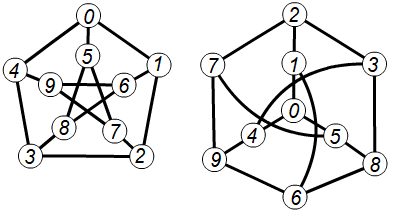
\includegraphics{chap1/fig1A1.png}
\end{figure}

(2)頂点集合を $\{1,2,3,4,5\}$の2元部分集合全体、辺集合を$\{(u,v) \mid u\cap v = \emptyset\}$ とするグラフ $G$ は注目しているグラフと同型である。
$G$ の自己同型群 $A$ は部分群として明らかに $S_5$ をもつ。
$A$ が $S_5$ と同型であることを示すために、$A$ の位数が120以下であることを示す。
固定化部分群を考えると、$A_{(1,2)}$ は $A$ の指数10の部分群である。
また$\Gamma((1,2))=\{(3,4),(3,5),(4,5)\}$であることから、$A_{(1,2),(3,4),(3,5),(4,5)}$ は $A_{(1,2)}$ の指数高々6の部分群である。
$A_{(1,2),(3,4),(3,5),(4,5)}$の位数は2であることが確かめられるので、$A$ の位数は高々 $10\times 6\times 2 =120$ である。
以上より示せた。

\subsection{}
連結成分 $C$ をとり,頂点数を $a$ とする.$C$ の頂点と $C'$ の頂点は辺で結ばれていないので,
辺の個数は $\comb{10}{2} - a(10-a)$ 以下である.$1\leq a\leq 9$ よりこの値は $36$ 以下であることが分かる.

ちょうど $36$ 本を実現することは可能である.$K_9$ にひとつの孤立点を加えたものが条件を満たす.

\subsection{}

\subsection{}

\subsection{}
頂点集合を$\{A_i\}$とし、辺集合を$\{(u,v)\mid |u \Delta v|=1\}$ とするグラフ $G$ を考える($\Delta$ は対称差)。
さらに各辺に対し $f:E(G)\to N: (u,v) \mapsto u\Delta v$ により色を定める($N$ の1元集合と $N$ の要素を同一視した)。
定義より、$u\setminus \{x\}=v\setminus \{x\}$ であることと、$u,v$ 間に色 $x$ の辺が存在することが同値である。
したがって、$S:=\{f(e) \mid e\in E(G)\}$ に含まれない $N$ の元が存在することを示せば良い。
もし $G$ が多角形を含むならば、その多角形には必ず同じ色の辺が偶数本ずつ含まれる。そのため、多角形から適当な辺を1つ取り除くことで、$S$ を変化させることなく、$G$ に含まれる多角形の個数を1つ以上減らすことができる。この操作を繰り返すことで $G$ は最終的に森になるが、このとき $|S|\leq |E(G)|<|V(G)|=n=|N|$ となり、示せた。

\subsection{}

\subsection{}

\subsection{}
$A = (a_{ij})_{i,j}$ とするとき,$A^2$ の $(i,j)$ 成分は $\sum_{k} a_{ik}a_{kj}$ である.
これは,$i$ から $j$ への長さ $2$ の歩道の個数と等しい.

\subsection{}

\subsection{}


\newpage

\section{ラベル付き木と数え上げ}
\subsection{}

\subsection{}
\prufer の校正における列 $(x,y) = ((x_1,ldots,x_{n-1}), (y_1,\ldots,y_{n-1})$ において,
各 $x_iy_i$ が木の辺に対応する.特に,頂点 $v$ の次数は $x_1,\ldots, x_{n-1}, y_1, \ldots, y_{n-1}$ における
$v$ の出現回数に等しい.

列 $x$ には $1,2,\ldots, n-1$ がちょうど一度ずつ現れる.よって,列 $y$ における $v$ の出現回数は $\deg(v) - 1$ に等しい.

以上の観察により,木 $T$ が本問の次数条件を満たすことは,その \prufer $P(T)$ において,
\begin{itemize}
 \item $2$ と $3$ が $2$ 度ずつ現れる.$5$ が $1$ 度現れる.他の数は現れない.
\end{itemize}
が成り立つことと同値である.木と \prufer の一対一対応より,木を数えることは,この条件を満たす数列の数え上げと等価で,
$\binom{5}{2,2,1} = 30$ 通りと計算できる.
\subsection{}

\subsection{}

\subsection{}
$n=9$ ならば,$1,9,2,8,3,6,4,5$ のように値を定める.
$n=10$ ならば,$1,10,2,9,3,8,4,7,5,6$ のように値を定める.
という要領で値を定めると,graceful labeling になることは容易に分かる.
\subsection{}

\subsection{}

\subsection{}


\newpage

\section{グラフの彩色とRamsey理論}
\subsection{}

\subsection{}
下界は定理3.2の系より直ちに明らか。そのような彩色の例として、$V(G)=\{0,1,2,3,4,5,6\}$ に対し、
\begin{align*}
(0,1),(1,2),(2,3),
(3,4),(4,5),(5,6),(6,0),
(1,4),(2,5),(3,6)
\end{align*}
を赤く、残りを青くするものが存在する。

\subsection{}
$a = N(p-1,q,2)$, $b = N(p,q-1;2)$ とする.
$n = a+b-1$ として,$K_n$ の辺を赤または青で塗る.赤の $K_p$ または青の $K_q$ がとれることを示せばよい.

赤い辺からなる部分グラフを $R$ とする.$n$ は奇数であり,奇点は偶数個であるから,$\deg_R(v)$ が偶数であるような $v$ が存在する.
$\deg_R(v) \geq a$ であるとき,その $a$ 個から赤い $K_{p-1}$ または青い $K_{q}$ がとれる.前者の場合 $v$ と合わせて赤い $K_p$ が得られ,
後者の場合そのまま青い $K_q$ が得られているので,この場合には示された.
$\deg_R(v) < a$ であるとする.$a$ と $\deg_R(v)$ はともに偶数なので,$\deg_R(v) \leq a-2$ が成り立つ.

青い辺からなる部分グラフを $B$ とすると,$\deg_B(v) = n - 1 - \deg_R(v) \geq b$ が成り立つ.よってこの場合も $\deg_R(v) \geq	a$ の場合と同様である.

\subsection{}
(1)
$N(4,4;2)\leq N(3,4;2)+N(4,3;2)=18$ であるので、$K_{17}$での反例を具体的に構築すれば良い。
$V(G)=\mathbb{Z}/17\mathbb{Z}$として、 
\begin{align*}
\text{辺} (i,j) \text{が赤} \Longleftrightarrow i-j = \pm 1,\pm 2,\pm 4,\pm 8
\end{align*}
とすればよい。

(2)
$N(3,5;2)\leq N(2,5;2)+N(3,4;2)=14$ であるので、$K_{13}$での反例を具体的に構築すれば良い。
$V(G)=\mathbb{Z}/13\mathbb{Z}$として、 
\begin{align*}
\text{辺} (i,j) \text{が赤} \Longleftrightarrow i-j = \pm 1,\pm 5
\end{align*}
とすればよい。

\subsection{}
\begin{enumerate}
 \item 不等式は $2^k\leq n$ と書き換えられる.
 
 $k$ についての帰納法で示す.$k=0$ はよい.$k\geq 1$ として $k-1$ での成立を仮定.$v_0\in K_n$ を任意にとる.
 \begin{align*}
  V_1 = \{w\mid \text{$v$ から $w$ へ向き付けられている}\},\\
  V_2 = \{w\mid \text{$w$ から $v$ へ向き付けられている}\}
 \end{align*}
 とすると,$|V_1| + |V_2| = n-1 \geq 2^{k}-1$ であるから,$V_1$ または $V_2$ のどちらかは $2^{k-1}$ 個以上の頂点を含む.
 その部分集合に帰納法の仮定を用いて $k-1$ 個の頂点からなる推移的トーナメントをとり,$v$ を合わせれば $k$ 個の頂点からなる推移的トーナメントが得られる.
 \item 不等式は $n^k < 2^{\comb{k}{2}}$ と言い換えられる.$n^k \geq \comb{n}{k}\cdot k!$ であるから,$\comb{n}{k}\cdot \frac{k!}{2^{\comb{k}{2}}} < 1$ が成り立つ.
 
 $K_n$ の各辺を,乱択で向き付けることを考える.$k$ 個の頂点集合に対して,それが推移的トーナメントになる確率は,$\frac{k!}{2^{\comb{k}{2}}}$ である(強い順に並べる方法が $k!$ 通りあり,
 向き付けの方法が $2^{\comb{k}{2}}$ 通りある).したがって,$\comb{n}{k}\cdot \frac{k!}{2^{\comb{k}{2}}}$ は,$k$ 個の頂点からなる推移的トーナメントの個数の期待値に等しい.
 この値が $1$ 未満であることから,ある向き付けに対して $k$ 個の頂点からなる推移的トーナメントの非存在が従う.
\end{enumerate}
\subsection{}

\subsection{}
頂点集合を$\{0,\ldots,n-1\}$とするクリーク $G$ の辺を、次のような $f:E(G)\to \{0,1\}^2$ により4色彩色する。
$$
f(\{i,j\})=(a_{xy},a_{yx}) \ \ (\text{ただし$x=\min(i,j),y=\max(i,j)$})
$$
このとき、Ramseyの定理から、$n$ 十分大なら、単色 $K_m$ が必ず存在する。そのような $K_m$ に属する頂点に対応する行および列からなる小行列が望むものである。

\subsection{}

\subsection{}
$V(G)=\mathbb{F}_{16}$ とする。$\mathbb{F}_{16}^*$ の生成元 $\alpha$ を取る。$G$ の辺の3色彩色 $f:E(G)\to \mathbb{Z}/3\mathbb{Z}$ を次で定める。

\begin{align*}
i-j = \alpha ^ n \text{ であるとき、 } f(\{i,j\}) = n \bmod 3
\end{align*}
(これはwell-definedであることに注意する)

この彩色が単色三角形を含まないことを背理法により示す。単色三角形ができたとし、その頂点を $i,j,k$ とする。等式 $k-i=(j-i)+(k-j)$ を定数倍することで
\begin{align*}
\alpha^6+\alpha^3+1=0 \text{ または } \alpha^9+\alpha^3+1=0
\end{align*}
が成り立つことがわかる。したがって$\mathbb{F}_2(\alpha^3)/\mathbb{F}_{2}$ の拡大次数は1,2,3,6のいずれかとなる。しかし、$\mathbb{F}_2(\alpha^3)$ は $\mathbb{F}_{16}$ の部分体であって、少なくとも6つの元 $\{0,1,\alpha^3,\alpha^6,\alpha^9,\alpha^{12}\}$ をもつことから、$\mathbb{F}_2(\alpha^3)=\mathbb{F}_{16}$であり、 $\mathbb{F}_{16}/\mathbb{F}_{2}$ の拡大次数は4であるので矛盾。

\subsection{}
このままだと $n=1$ で自明に嘘だったので, $k> \sqrt{2n} - 1$ で示します.

赤三角形のない極大誘導部分グラフを $H$ とする(空集合を頂点集合とする誘導部分グラフが条件を満たすので,極大なものは存在する).
任意の $v\in G-H$ に対して,$H+v$ が赤三角形を含む.したがって,$e=ab\in H$ であって,$ab, av, bv$ がすべて赤いものが存在する.
このような $e$ をひとつとり $f(v)$ とすることで,写像 $f\colon V(G-H) \longrightarrow E(H)$ を定める.

問題の条件(同一の辺が $2$ 個の赤三角形に含まれない)から,$f$ は単射である.したがって $|V(G-H)| \leq |E(H)|$.
$|V(H)| = k$ とすると,$n - k\leq \binom{k}{2}$ となる.
$2n \leq k(k+1)$ より $\sqrt{2n} < k+1$ となり $k > \sqrt{2n} - 1$ が分かる.

\subsection{}
$G$ を $d$ 色で彩色する.最も少ない回数使われた色が $1$ であるとしてよい(特に,色 $1$ の頂点は $\frac{n}{d}$ 以下である).
各色 $1$ の頂点 $v$ に対して,まわりには色 $2,\ldots,d$ のいずれかの色の頂点が合計で $d$ 個以下ある.
$2(d-1) > d$ であるから,ある色は $v$ の隣接点に $1$ 度しか現れていない.そのような頂点を $w_v$,色を $c_v$ とする.

$G$ を次のように変形すれば $d-1$ 色での彩色が得られる:
各 $v$ に対して辺 $vw_v$ を除く.$v$ の色を $c_v$ に変更する.

色 $1$ の取り方によりこの過程で除かれる辺の数は $\frac{n}{d}$ 以下であるからよい.

\newpage

\section{Tur\'{a}nの定理と極値グラフ}
\subsection{}

\subsection{}
帰納法.$n$ について示されたとして,$n+2$ の場合に示す.
$G$ を $n+2$ 頂点かつ辺が $\lfloor \frac{(n+2)^2}{4}\rfloor$ 本とする.隣接する $2$ 点 $a,b$ をとり,$G_1 = G\setminus \{a,b\}$ とする.

$G_1$ は三角形を含まないので,$|E(G_1)|\leq \lfloor\frac{n^2}{4}\rfloor$.
また三角形の非存在より,各 $v\in V(G_1)$ は $a,b$ のうち高々一方としか隣接していない.よって $G_1$ と $\{a,b\}$ の間にある辺の本数は $|V(G_1)| = n$ 本以下.
したがって,$|E(G)|\leq \lfloor\frac{n^2}{4}\rfloor + n + 1$ が成り立つ.

$|E(G)|$ に対する仮定よりこの不等式において等号が成り立つ.よって議論に用いた不等式評価は全て最善であるから,
$|E(G_1)| = \lfloor\frac{n^2}{4}\rfloor$ であり,各 $v\in V(G_1)$ は$a,b$ のうちちょうど一方と隣接する.
このことと帰納法の仮定より,まず $G_1$ が $K_{k,k}$ あるいは $K_{k,k+1}$ であることが分かり,三角形ができないという条件から $v$ と $a,b$ の結び方も決まって $G$ に対する主張が従う.
\subsection{}
まず辺 $a=\{x,y\}$ を含む三角形を下から評価する.
$A = \Gamma(x)\setminus y$, $B=\Gamma(x)\setminus y$ とする.$|A| = \deg(x) - 1$, $|B| = \deg(y) - 1$, $A,B\subset G\setminus\{x,y\}$ である.
よって $|A\cap B| = |A| + |B| - |A\cup B| \geq (\deg(x)-1) + (\deg(y)-1) - (n-2) = \deg(x) + \deg(y) - n$ である.
特に辺 $a$ を含む三角形は $\deg(x) + \deg(y) - n$ 個以上存在する.

辺 $e$ と三角形 $T$ の組 $(e,T)$ であって,$e\subset T$ となるものの個数を $2$ 通りに数える.
まず $T$ から $e$ を数えることで,個数は $3\Delta$ (ただし $\Delta$ は三角形の個数).
また上で示したことを使って $e$ から $T$ を数えることで,個数は
$\sum_{a=xy}(\deg(x)+\deg(y)-n)$ 以上.したがって
\[
 \Delta\geq \frac13\sum_{a=xy}(\deg(x)+\deg(y)-n)
\]
が分かる.

この右辺は $\frac13\sum_{a=xy}(\deg(x)+\deg(y)-n)=\frac13\bigl(\sum_x \deg(x)^2 - n^2)$ と評価できる.
さらに握手補題とコーシー・シュワルツの不等式より
$\sum_x \deg(x)^2 \leq \frac1n (\sum_x\deg(x))^2 = \frac{(2e)^2}{n}$ であり,これらを合わせて主張の不等式を得る.

\subsection{}

\subsection{}

\subsection{}

\subsection{}
Mantel の証明のほぼ単純な拡張である.
各頂点 $v$ に非負の重み $z_v$ (全頂点の重みの和は $1$)を与えて,$\sum_{e=ab}z_az_b$ の最大値が達成されている状況を考える.
そのうち,正の重みの頂点数が最小のものをとると,正の重みの頂点数が $p-1$ 以下であることが分かる
($p$ 個以上あれば,クリークの非存在より非隣接点に正の重みが乗っていて,それをまとめて頂点数が減らせる).

$k = p-1$ とし,それらの重みを $z_1,\ldots,z_k$ とする.
$\sum_{i\neq j}z_iz_j = \frac12((z_1+\cdots+z_k)^2 - (z_1^2+\cdots+z_k)^2)$ であるが,コーシー・シュワルツの不等式などから
$z_1^2+\cdots+z_k^2 \geq \frac{1}{k}(z_1+\cdots+z_k)^2$ が分かるので,$z_1+\cdots+z_k=1$ と合わせて $\sum_{i\neq j}z_iz_j \leq \frac12(1-\frac{1}{k})$ である.

最大値を達成する割り当てでこの不等式が成り立つので,任意の割り当てでも成り立つ.特に全頂点に重み $\frac{1}{n}$ を割り当てたときのことを考えて
$\frac{|E(G)|}{n^2}\leq \frac{1}{2}(1-\frac{1}{k})$ が成り立つ.これに $k=p-1$ を代入して整理すればよい.
\subsection{}



\newpage

\section{個別代表系}
\subsection{}

\subsection{}

\subsection{}

\subsection{}

\subsection{}

\subsection{}
各 $A_i$ から要素 $a_i\in A$ を一様に乱択する.
$(a_1,\ldots,a_n)$ が代表系となるよう確率が正であることを示せばよい.

$i < j$ に対して確率変数 $X_{ij}$ を,$a_i = a_j$ のときに $1$,そうでないとき $0$ として定める.
期待値は $E(X_{ij}) = P(a_i=a_j) = \frac{A_i\cap A_j|}{|A_i|\cdot|A_j|}$ である.

$X = \sum_{ij} X_{ij}$ とすると,$E(X) = \sum_{ij}E(X_{ij})$ であるが,$E(X_{ij})$ の計算と問題の仮定より,$E(X) < 1$ である.
したがって $P(X<1) > 0$ となるので,$X<1$ となる選び方 $(a_1,\ldots,a_n)$ が存在する.これは代表系である.
\subsection{}
$2n$ 頂点の $(n-1)$-正則二部グラフ $G_n$ をとる.(1), (2) ではこれの $n=4, 5$ の場合が問題となっている.

$G_n$ は完全二部グラフ $K_{n,n}$ の部分グラフと見なせる.よって $K_{n,n}$ から完全マッチングをひとつ除いたものと見なせる.
よって頂点の名前を上手く付けることで,
\begin{itemize}
 \item $G_n$ は部集合 $A = \{v_1,v_2,\ldots,v_n\}$, $B = \{w_1,w_2,\ldots,w_n\}$ を持つ二部グラフ.
 \item $v_iw_j\in G_n \iff i \neq j$.
\end{itemize}
が成り立つ(特に $G_n$ は同型を除き一意に定まる).

完全マッチングは,$\{v_iw_j\}$ に対して写像 $f\colon i\mapsto j$ を対応させることで,完全マッチングは
不動点を持たない全単射 $f\colon \{1,2,\ldots,n\}\longrightarrow  \{1,2,\ldots,n\}$ と一対一に対応する.

この数え上げは,完全順列(攪乱順列)の数え上げとして有名である.
答は $\sum_{k=0}^n (-1)^k\frac{n!}{k!}$ であり,(1), (2) の答は $n=4, 5$ の場合 (1)9, (2)44 である.

\newpage

\section{Dilworthの定理と極値集合論}
\subsection{}

\subsection{}

\subsection{}

\subsection{}

\subsection{}



\end{document}